\chapter{Complexité du dénombrement}
\label{cha:complexite-du-denombrement}

Qu'est-ce qu'un problème de dénombrement? Simplement, un tel problème consiste à compter le nombre de solutions respectant un ensemble de contraintes. Les problèmes de dénombrement, ou de comptage, font partie des problèmes computationnels difficiles, c'est-à-dire qu'il est peu probable qu'ils soient résolubles efficacement. Les problèmes de comptage surgissent dans de nombreuses disciplines, avec des applications en raisonnement probabiliste~\cite{rothHardnessApproximateReasoning1996, sangPerformingBayesianInference2005, abramsonHailfinderBayesianSystem1996}, en fiabilité des réseaux~\cite{valiantComplexityEnumerationReliability1979, duenas-osorioCountingbasedReliabilityEstimation2017}, en mécanique statistique~\cite{jerrumPolynomialTimeApproximationAlgorithms1993} et en intelligence artificielle~\cite{balutaQuantitativeVerificationNeural2019}. Contrairement à certains problèmes étudiés dans le domaine du calcul quantique, tels que l'échantillonnage de bosons~\cite{aaronsonComputationalComplexityLinear2011} ou l'échantillonnage de circuits aléatoires~\cite{boulandComplexityVerificationQuantum2019}, une solution à ces problèmes peut avoir un impact concret, justifiant alors l'étude de tels problèmes. Par exemple, les problèmes de comptage permettent d'estimer la fiabilité des réseaux de transmission d'énergie~\cite{duenas-osorioCountingbasedReliabilityEstimation2017} ou d'analyser la sécurité des réseaux de neurones~\cite{balutaQuantitativeVerificationNeural2019}.

Ce chapitre décrit le cadre théorique entourant la classe des problèmes de dénombrement en détail. Pour ce faire, celle-ci est définie à l'aide du langage de la théorie de la complexité à la section~\ref{sec:classes-de-complexite}. Le problème de comptage prototypique, le problème de satisfaisabilité, sert d'exemple et est décrit à la section~\ref{sec:satisfaisabilite-booleenne}. Celui-ci est d'une grande importance pour ce projet et est ainsi référencé tout au long de ce mémoire. La section~\ref{sec:intractabilite-approximation-et-optimisation} explique l'importance des méthodes approximatives alors que la section~\ref{sec:comptage-de-modeles} décrit les solveurs modernes pour les problèmes de comptage. Finalement, le comportement des instances aléatoires de ces problèmes est présenté à la section~\ref{sec:transitions-de-phase}, où des transitions de phase font étonnamment leurs apparitions.

Il est souvent favorable de décrire la théorie de la complexité à l'aide du concept de \textit{machine de Turing}. Cependant, ce mémoire suppose que la thèse de Church-Turing soit vraie, et donc que n'importe quel modèle de calcul puisse être utilisé de manière équivalente, pour faire abstraction de ce langage et simplifier les idées présentées.

%-----------------------------------------------------------------------------%

\section{Classes de complexité}
\label{sec:classes-de-complexite}

La théorie de la complexité s'intéresse à la classification des problèmes algorithmiques en \textit{classes de complexité}, c'est-à-dire en ensembles de problèmes de même complexité. Classifier un problème permet de caractériser les ressources nécessaires pour sa résolution par un algorithme. Les problèmes d'une même classe ont une difficulté intrinsèque similaire, ce qui facilite le choix d'un algorithme et de ressources appropriées. Savoir qu'un problème n'est pas réalistement résoluble, ou plus précisément intraitable, limite les attentes. Sachant ceci, la recherche dans cette direction s'avère grandement utile. La théorie de la complexité cherche aussi à comparer les problèmes de différentes complexités pour comprendre l'espace des problèmes en plus grande profondeur. Comparer des problèmes faciles avec des problèmes difficiles peut par exemple aider à comprendre ce qui rend un problème difficile et donc à trouver des algorithmes résolvant efficacement les problèmes plus complexes. Des liens, nommés réductions, sont définis entre différents problèmes pour comparer leurs complexités. Un algorithme efficace pour un problème peut en effet être efficace pour un différent problème s'il existe une réduction entre ceux-ci. Les classes de complexité, de manière similaire au modèle de la machine de Turing, tentent de définir de manière abstraite la difficulté d'un problème. Quel que soit le matériel informatique à notre disposition, un problème d'une classe donnée ne doit pas changer de classe; un problème simple doit rester simple dans tous les cas.

Comment est-il possible de déterminer la complexité d'un problème? Pour ce faire, les classes de complexité se basent sur les ressources indispensables à la résolution du problème: le temps et la mémoire. Afin de trouver la solution à un problème, un programme doit effectuer un certain nombre d'opérations, limité dans le temps par le matériel informatique. On parle alors de \textit{complexité en temps}. Afin de produire un résultat final, le programme doit aussi garder en mémoire les résultats intermédiaires. Ceux-ci doivent être sauvegardés dans le matériel informatique afin d'être réutilisés ultérieurement. Comme la quantité d'information conservée est aussi un facteur limitant pour le matériel informatique, on parle donc de \textit{complexité en espace}. 

La complexité en temps et en espace d'un problème est définie selon la taille de celui-ci. Afin de capturer cette dépendance, une loi d'échelle est utilisée pour encapsuler la difficulté d'un problème en fonction de sa taille. Le temps et la mémoire quantifient bien les ressources nécessaires des algorithmes. Par contre, ceux-ci dépendent du matériel informatique utilisé. Il est attendu qu'un ordinateur moderne soit bien plus performant qu'une des premières machines analogues. Comment retirer cette dépendance de la notion de complexité? Pour ce faire, on fait appel à la notation asymptotique, communément appelée la \textit{notation $\mathcal{O}$}. La notation asymptotique caractérise la vitesse de croissance d'une fonction en ne considérant que son comportement global à l'infini. Les coefficients ainsi que les termes asymptotiquement inférieurs ne sont pas considérés. Par exemple, pour un problème de taille $n$, la résolution de celui-ci pourrait demander un temps exponentiel $\mathcal{O}(2^{n})$ et une mémoire polynomiale $\mathcal{O}(n)$. Remarquons qu'il n'y a aucune dépendance au matériel informatique; deux ordinateurs différents doivent effectuer le même nombre d'opérations et sauvegarder la même quantité d'information. Un de ces ordinateurs pourrait toutefois résoudre le problème plus rapidement si celui-ci peut effectuer un plus grand nombre d'opérations par seconde ou accéder plus rapidement à sa mémoire. L'attrait des classes de complexité vient donc en partie de cette abstraction du matériel informatique.

La quantification de ces ressources permet la séparation de plusieurs problèmes: il est en effet souhaitable de séparer les algorithmes efficaces de ceux qui ne le sont pas. Commençons par définir deux classes de complexité particulièrement importantes: \textsf{P} et \textsf{NP}. Pour ce faire, un certain type de problème doit d'abord être défini. Un \textit{problème de décision} regroupe simplement tous les problèmes pouvant se répondre par « oui » ou « non ». Tout problème de décision $A$ peut être représenté par une fonction $A(x) \in \set{ 0, 1 }$, où $x$ désigne une instance du problème. Plus précisément, si la réponse à l'instance $x$ est « oui », alors $A(x)=1$; sinon $A(x)=0$. Les problèmes de décision se manifestent fréquemment, tant en informatique qu'en physique. Ceux-ci se présentent sous diverses formes: est-ce qu'un nombre $x$ est premier? La configuration $x$ représente-t-elle un état fondamental du système donné? Est-ce qu'il existe un chemin $x$ parcourant une seule fois toutes les villes d'une région en parcourant au maximum une distance $d$?

Quand peut-on dire qu'un problème de décision est résoluble efficacement? La classe de complexité \textsf{P}, pour « temps polynomial », tente de répondre à cette question. Informellement, un problème de la classe \textsf{P} est un problème de décision qui peut être résolu en temps polynomial. Un problème est donc considéré comme efficacement résoluble ou \textit{traitable}, s'il appartient à la classe \textsf{P}. 

\begin{maindefinition}{Classe de complexité \textsf{P}}{classe-p}
    Une fonction $A$ fait partie de la classe de complexité \textsf{P} si et seulement si $A(x)$ est calculable en temps polynomial, c’est-à-dire en temps $O(n^{c})$, où $n = \lvert x \rvert$ et $c$ est une constante.
\end{maindefinition}

Soit, par exemple, le problème de décision du test de primalité $A$. Ce problème cherche à déterminer si un entier naturel $x$ de taille $n=\lvert x \rvert $ est premier ou composé. Il peut être résolu, c'est-à-dire qu'il est possible de calculer $A(x)$, en temps polynomial $\tilde{O}(\log(n)^{12})$~\cite{agrawalPRIMES2004}, où la notation $\tilde{O}$ signifie que les termes polylogarithmiques sont aussi cachés. 

La relation entre un calcul en temps polynomial et un calcul efficace semble évidente de prime abord. La thèse de Cobham–Edmonds indique en effet qu'un problème algorithmique peut être résolu efficacement s'il est résoluble en temps polynomial~\cite{cobhamIntrinsicComputationalDifficulty1965, edmondsPathsTreesFlowers1965}. Cependant, certains problèmes ne possèdent pas de solutions trouvables efficacement en pratique. Par exemple, un problème peut appartenir à la classe \textsf{P}, mais être doté d'un grand coefficient limitant le calcul. Cela n'étant pas le cas pour la majorité des problèmes, cette supposition s'avère malgré tout une bonne règle empirique. 

Une deuxième classe particulièrement importante en théorie de la complexité est la classe \textsf{NP}, pour « temps polynomial non déterministe ». Celle-ci regroupe les problèmes de décision dont les solutions sont vérifiables en temps polynomial. Généralement, ces problèmes sont formulés sous la forme suivante: existe-t-il une solution, vérifiable en temps polynomial, au problème donné? Bien que les solutions soient vérifiables efficacement, déterminer l'existence d'une telle solution n'est pas nécessairement possible en temps polynomial. Une métaphore souvent utilisée pour la description d'un problème \textsf{NP} est celle d'une aiguille dans une botte de foin. Trouver cette aiguille parmi la quantité énorme de brins de foin est un défi de taille. Par contre, une fois l'aiguille trouvée, il n'y a aucun doute qu'il s'agit bien d'une aiguille. 

\begin{maindefinition}{Classe de complexité \textsf{NP}}{classe-np}
    Une fonction $A$ fait partie de la classe de complexité \textsf{NP} si et seulement si elle prend la forme
    \begin{equation*}
        A(x) = \exists y \mid B(x,y)
    \end{equation*}
    pour une fonction $B \in  \textsf{P}$, où $\lvert y \rvert = \mathrm{poly}(\lvert x \rvert)$.
\end{maindefinition}

Le symbole $\exists$ (« il existe ») désigne le quantificateur existentiel et  implique l'existence d'un objet $x$ satisfaisant une propriété $P(x)$ donnée. La notation $\exists x \mid P(x)$ signifie donc qu'il existe un objet $x$ tel que la propriété $P(x)$ est satisfaite. La fonction $B$ est appelée le vérificateur du problème de décision $A$ et $y$ le certificat, ou le témoin, associé à l'entrée $x$. La définition précédente pose alors la question de l'existence d'un certificat $y$, ou autrement dit d'une solution à l'entrée $x$, vérifiable en temps polynomial par une fonction $B$. Un exemple de problème \textsf{NP} est le problème de décision du commis voyageur. Soit un graphe $x$ représentant les villes d'une région particulière. Est-ce que le commis voyageur peut visiter toutes les villes exactement une fois et revenir à son point de départ en parcourant une distance inférieure à $d$? Dans ce cas, la fonction $A$ détermine s'il existe un tel chemin alors que la fonction $B$ détermine si le chemin $y$ est de taille inférieure à $d$.

La classe \textsf{NP} est également définie comme la classe de problèmes que peut résoudre une machine de Turing non déterministe en temps polynomial, d'où son nom. Cette définition est toutefois équivalente à la définition précédente, c'est-à-dire la classe de problèmes vérifiable par une machine de Turing déterministe en temps polynomial~\cite{sipserIntroductionTheoryComputation1996}. Notons que la classe \textsf{P} est contenue dans la classe \textsf{NP}. En effet, comme un problème de \textsf{P} est résoluble en temps polynomial, alors nécessairement une solution à ce problème peut aussi être vérifiée en temps polynomial. Cependant, une question, faisant partie des problèmes du prix du millénaire~\cite{carlsonMillenniumPrizeProblems2006}, demeure ouverte: est-ce que $\textsf{P} = \textsf{NP}$? La conjecture la plus largement répandue répond à cette question par la négative. L'hypothèse de temps exponentiel~\cite{impagliazzoComplexityKSAT2001} suggère par exemple que certains problèmes de \textsf{NP} sont résolubles en temps exponentiel, un résultat significatif sur la difficulté de ces problèmes. En conséquence, un problème est \textit{intraitable} s'il n'est pas résoluble en temps polynomial, par opposition à un problème traitable. 

La classe de complexité d'intérêt dans le cadre de ce mémoire est la classe \textsf{\#P} introduite par Valiant~\cite{valiantComplexityComputingPermanent1979}. Cette classe, définie par extension à la classe \textsf{NP}, cherche non seulement à déterminer si un problème de décision possède une solution, mais aussi à spécifier le nombre de solutions à ce problème. Ainsi, un \textit{problème de dénombrement} ou un \textit{problème de comptage} consiste à trouver le nombre de solutions d'un problème de décision. Un problème de comptage est donc défini par rapport à un problème de décision. Prenons par exemple le problème du commis voyageur. Le problème de décision généralement défini cherche un trajet de taille inférieure à une certaine distance. Le problème de comptage adjoint exige alors le nombre de trajets possibles de taille inférieure à la distance donnée. 

\begin{maindefinition}{Classe de complexité \textsf{\#P}}{classe-sharp-p}
    Une fonction $A$ fait partie de la classe de complexité $\textsf{\#P}$ si et seulement si elle prend la forme
    \begin{equation*}
        A(x) = \lvert \set{ y \mid B(x, y)} \rvert
    \end{equation*}
    pour une fonction $B \in \textsf{P}$, où $\lvert y \rvert = \mathrm{poly}(\lvert x \rvert)$ pour toutes les valeurs $y$ prises par $B(x,y)$.
\end{maindefinition}

Par définition, un problème de la classe \textsf{\#P} est au moins aussi difficile qu'un problème de la classe \textsf{NP}. Connaître le nombre de solutions à un problème de décision indique effectivement s'il existe au moins une solution à un problème de décision. Cependant, les problèmes de comptage intéressants possèdent fréquemment un nombre exponentiel de solutions, impliquant une plus grande complexité inhérente.

Comme que les problèmes de la classe \textsf{P} appartiennent aussi à la classe \textsf{NP}, et que les problèmes de cette dernière appartiennent aussi à la classe \textsf{\#P}, il est nécessaire de définir un concept supplémentaire spécifiant la difficulté d'un problème au sein d'une classe. Intuitivement, un problème est \textit{difficile} pour une classe de complexité s'il est au moins aussi difficile que tous les problèmes de la classe. Plus formellement, un problème difficile pour une classe donnée signifie qu'il existe une réduction en temps polynomiale de tous les problèmes de la classe au problème difficile. Une \textit{réduction en temps polynomial} d'un problème à un autre signifie qu'il est possible d'utiliser le second problème pour résoudre le premier au coût d'un facteur polynomial. De plus, un problème est \textit{complet} s'il est difficile et aussi membre de la classe. La figure~\ref{fig:complexity-classes} éclaircit ces concepts. Les problèmes complets d'une classe représentent alors les problèmes les plus difficiles de celle-ci. Par exemple, le problème de décision associé au problème du commis voyageur est dit \textsf{NP}-complet, car il fait partie des problèmes considérés comme difficiles de la classe \textsf{NP}. Il est toutefois cru que celui-ci ne fasse pas partie de la classe \textsf{P} selon la conjecture $\textsf{P} \neq \textsf{NP}$.

\begin{figure}[h]
    \centering
    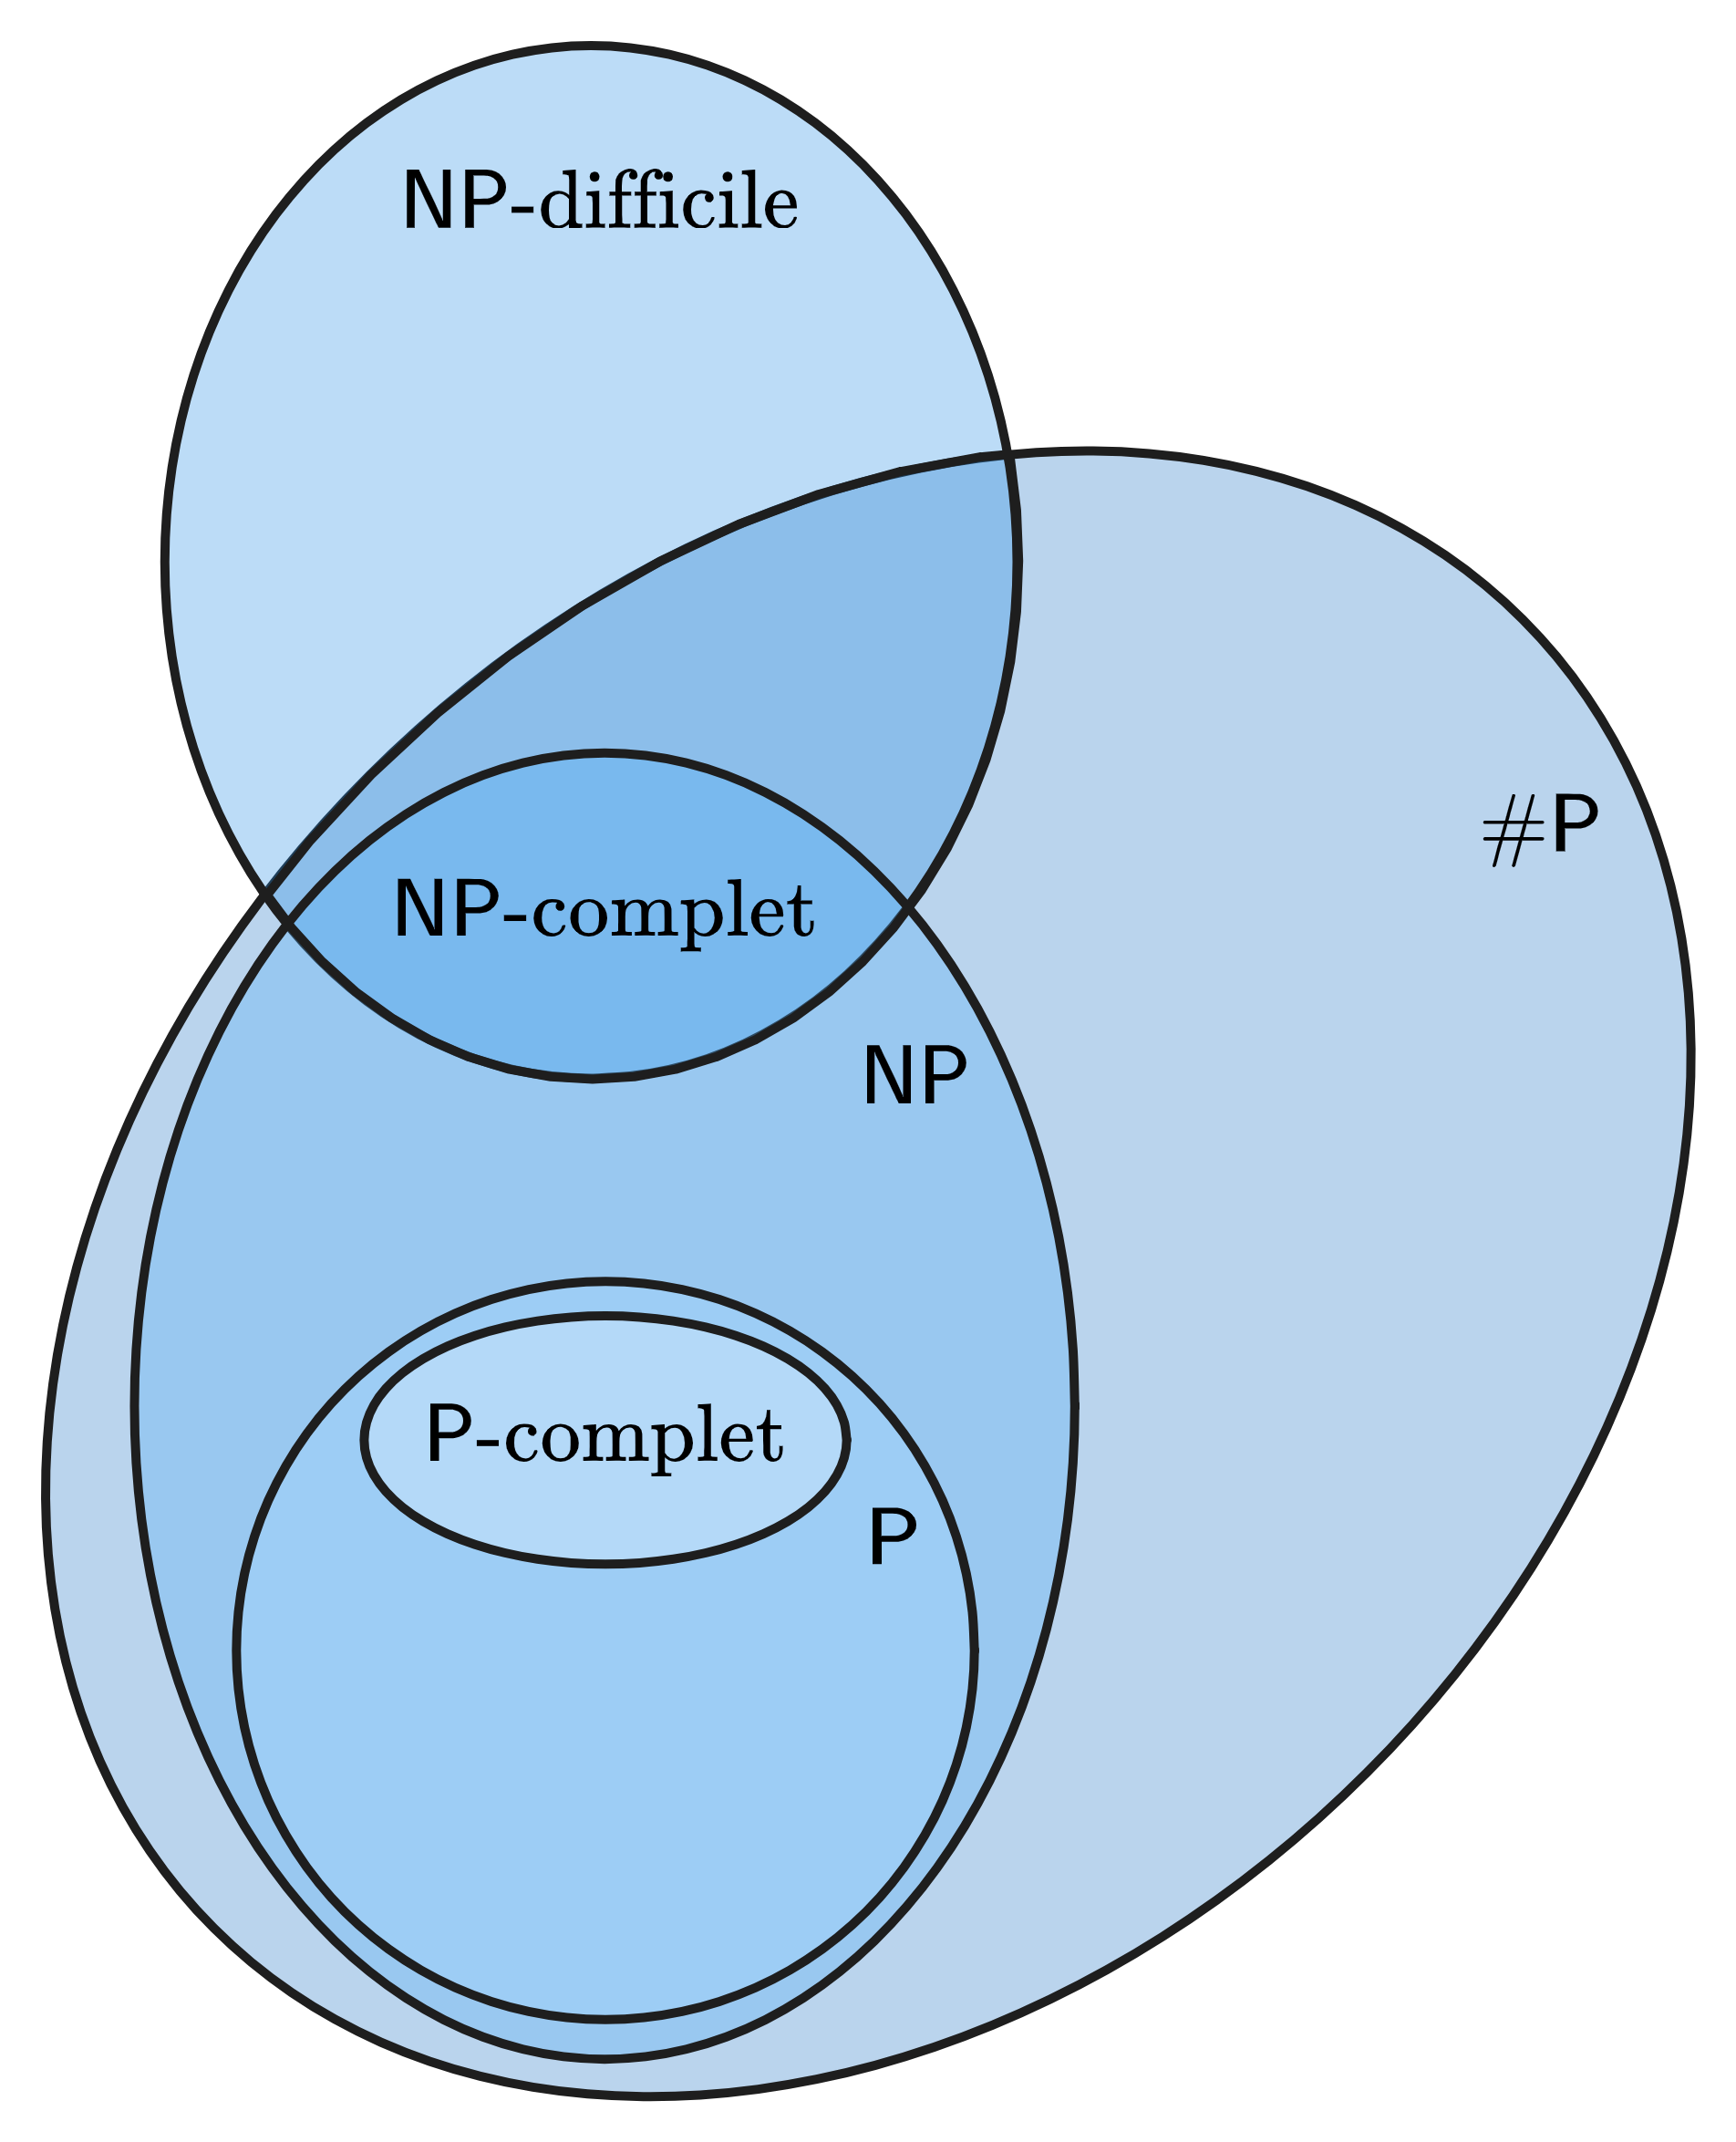
\includegraphics[width=0.35\textwidth]{figures/complexity-classes.png}
    \caption[Classes de complexité]{Schéma de différentes classes de complexité. Cette illustration suppose la conjecture $\textsf{P} \neq \textsf{NP}$. Pour plus de rigueur, la classe \textsf{\#P} devrait être remplacée par la classe $\textsf{P}^{\textsf{\#P}}$.}
    \label{fig:complexity-classes}
\end{figure}

L'importance des problèmes \textsf{\#P} au sein de la théorie de la complexité s'observe entre autres par le théorème de Toda~\cite{todaPPHardPolynomialTime1991}. Ce résultat marquant montre que tous les problèmes de la hiérarchie polynomiale \textsf{PH} peuvent être résolus en temps polynomial avec un oracle \textsf{\#P}, c'est-à-dire avec une boîte noire résolvant instantanément les problèmes de la classe \textsf{\#P}. Qu'est-ce que la hiérarchie polynomial \textsf{PH}? Celle-ci généralise les classes de complexité \textsf{P}, \textsf{NP} et \textsf{co-NP} en capturant les classes de problèmes exprimés par une alternance de quantificateurs d'existence ($\exists$, « il existe ») ou d'universalité ($\forall$, « pour tout »). La classe \textsf{co-NP} est la classe complémentaire à la classe \textsf{NP} et comprend en conséquence tous les problèmes dont les non-solutions sont vérifiables en temps polynomial. Celle-ci peut être définie, de manière similaire à la définition~\ref{def:classe-np}, à l'aide du complément du quantificateur d'existence $\exists$: le quantificateur d'universalité $\forall$. La classe \textsf{P}, définie sans quantificateur, est située au premier niveau de la hiérarchie \textsf{PH}, alors que les classes \textsf{NP} et \textsf{co-NP}, définies respectivement avec les quantificateurs $\exists$ et $\forall$, sont situées au deuxième niveau. Une infinie de classes peuvent être définies en combinant les différents quantificateurs, menant ainsi à une hiérarchie. Autrement dit, le théorème de Toda signifie que la hiérarchie \textsf{PH} est comprise dans la classe de complexité $\textsf{P}^{\textsf{\#P}}$, c'est-à-dire la classe de problèmes résolubles en temps polynomial avec un oracle \textsf{\#P}. Comme la hiérarchie polynomiale contient un immense nombre de différentes classes, chacune contenant des problèmes intéressants, ce théorème suggère l'incroyable puissance des problèmes de comptage.

\begin{subtheorem}{Théorème de Toda}{toda}
    La hiérarchie polynomiale \textsf{PH} est contenue dans $\textsf{P}^{\textsf{\#P}}$.
\end{subtheorem}

L'ordinateur quantique bouleverse le domaine de la complexité classique. Les problèmes autrefois intraitables deviennent potentiellement résolubles efficacement à l'aide d'algorithmes quantiques. Deux nouvelles classes de complexité font alors leurs apparitions pour décrire les problèmes résolubles à l'aide de matériel informatique quantique. La classe \textsf{BQP} généralise la classe \textsf{BPP} pour les ordinateurs quantiques, où la classe \textsf{BPP}, pour « temps polynomial probabiliste à erreur bornée », est l'ensemble des problèmes résolubles par un algorithme stochastique avec une probabilité d'erreur inférieure à $1/3$. De plus, la classe de complexité \textsf{QMA}, pour « Merlin Arthur Quantique » se définit par rapport à la classe \textsf{BQP} de manière analogue à la classe \textsf{NP} pour la classe \textsf{P}. La théorie de la complexité quantique étudie les classes de complexité quantiques dans l'objectif de déterminer les problèmes où les algorithmes quantiques présentent un avantage par rapport aux algorithmes classiques. Ce mémoire avance la recherche dans cette direction en étudiant la différence en performance des algorithmes quantiques et des algorithmes classiques.

%-----------------------------------------------------------------------------%

\section{Satisfaisabilité booléenne}
\label{sec:satisfaisabilite-booleenne}

Le problème de \textit{satisfaisabilité booléenne} ou problème SAT est particulièrement important dans la théorie de la complexité. Montré comme \textsf{NP}-complet par le théorème de Cook-Levin~\cite{cookComplexityTheoremprovingProcedures1971,levinUniversalSequentialSearch1973}, il fut à la base de la définition de \textsf{NP}-complétude et du problème $\textsf{P} \stackrel{?}{=} \textsf{NP}$. Celui-ci est aussi couramment utilisé dans la preuve de réductions de problèmes au sein de la classe de complexité \textsf
{NP}. Le problème SAT a une multitude d'applications, comme le diagnostic des fautes d'un circuit logique ou la planification en intelligence artificielle~\cite{marques-silvaPracticalApplicationsBoolean2008}, en partie grâce à la facilité de formuler ces applications à l'aide de formules propositionnelles.

Une \textit{formule propositionnelle}, ou une expression booléenne, est un ensemble de variables booléennes $x_{i} \in \set{\textsc{\texttt{FAUX}}, \textsc{\texttt{VRAI}}}$ reliées par des opérateurs booléens de conjonctions (\textsc{\texttt{OU}}, $\lor$), de disjonctions (\textsc{\texttt{ET}}, $\land$) ainsi que de négation (\textsc{\texttt{NON}}, $\neg$).  Un \textit{littéral} désigne dans ce contexte une variable booléenne ou sa négation. Par exemple, l'expression $(x_{1} \land x_{2}) \lor \neg x_{3}$ est une formule booléenne composée des variables $x_{1}$, $x_{2}$ et $x_{3}$, ainsi que des littéraux $x_{1}$, $x_{2}$ et $\neg x_{3}$. Notons que l'équivalence $\textsc{\texttt{FAUX}} \leftrightarrow 0$ et $\textsc{\texttt{VRAI}} \leftrightarrow 1$ est utilisée dans ce mémoire par commodité.

Un problème SAT se décrit par une formule propositionnelle. Résoudre le problème consiste à déterminer s'il existe une combinaison de variables qui rend la formule logiquement vraie, c'est-à-dire que l'évaluation de celle-ci donne 1. Une telle formule est alors dite satisfaisable.

\begin{maindefinition}{Problème SAT}{probleme-sat}
    Soit une constante $n \geq 1$ et une formule propositionnelle $\varphi(x_{1}, x_{2}, \dots, x_{n})$ où $x_{i} \in \set{ 0, 1 }$.  Existe-t-il une assignation des variables $x_{1}, x_{2}, \dots, x_{n}$ pour laquelle l'expression $\varphi$ soit satisfaisable, c'est-à-dire que $\varphi(x_{1}, x_{2}, \dots, x_{n})=1$?
\end{maindefinition}

Dans l'étude du problème SAT, les formules propositionnelles sont souvent exprimées en \textit{forme normale conjonctive} (« Conjunctive Normal Form ») (CNF). On parle alors de formules CNF. Celles-ci consistent en une conjonction d'une ou de plusieurs \textit{clauses}, où une clause est une disjonction d'un ou plusieurs littéraux. Cela implique que toute clause doit contenir au moins un littéral évaluant à 1 pour que la formule soit satisfaisable. Toute formule propositionnelle peut être réécrite en forme normale conjonctive en utilisant les lois de l'algèbre booléenne.

\begin{example}{Problème SAT}{probleme-sat}
    La formule CNF
    \begin{equation*}
        \varphi(x_{1}, x_{2}, x_{3}) = (x_{1} \lor x_{3}) \land (\neg x_{1} \lor x_{2} \lor \neg x_{3})
    \end{equation*}
    est satisfaisable car $\varphi(1,0,0) = (1 \lor 0) \land (\neg 1 \lor 0 \lor \neg 0) = 1$. Au contraire, la formule CNF
    \begin{equation*}
        \varphi(x_{1})= (x_{1}) \land (\neg x_{1})
    \end{equation*}
    n'est pas satisfaisable car $\varphi (x_{1}) = 0$ peu importe le choix de $x_{1}$.
\end{example}

Le problème kSAT constitue un cas spécial du problème SAT où le nombre de littéraux appartenant à chaque clause d'une formule CNF est restreint à $k$ littéraux au maximum. Notons que le problème kSAT est trivial pour $k=1$, résoluble en temps linéaire pour $k=2$~\cite{kromDecisionProblemClass1967}, et \textsf{NP}-complet pour $k \geq 3$~\cite{karpReducibilityCombinatorialProblems1972}. Surprenamment, les problèmes de comptage correspondants, \#2SAT et \#3SAT, appartiennent tous deux à la classe \textsf{\#P}-complet~\cite{valiantComplexityEnumerationReliability1979}. Ainsi, compter le nombre de solutions à un problème \textsf{NP}-complet peut être difficile même s'il est possible de trouver une solution efficacement. Intuitivement, cette difficulté provient du nombre exponentiel de solutions que possèdent les problèmes \#2SAT et \#3SAT.

Dans ce mémoire, deux variantes de 3SAT sont portées à l'étude: le problème Pas-Tous-Égaux 3SAT (« Not-All-Equal 3-Satisfiability ») (NAE3SAT) et le problème 1-dans-3 3SAT (« One-in-Three 3-Sastisfiability ») (1-in-3SAT). 
Comme le problème SAT, ces problèmes appartiennent aussi à la classe de complexité \textsf{NP}-complet. Les versions monotones de ces problèmes, où la négation de variables n'est pas permise, sont étonnamment aussi \textsf{NP}-complet par le théorème de dichotomie de Schaefer~\cite{schaeferComplexitySatisfiabilityProblems1978}. Ces problèmes de décision peuvent être associés aux problèmes de comptage \#NAE3SAT et \#1-in-3SAT de la classe de complexité \textsf{\#P}.

\begin{maindefinition}{Problème NAE3SAT}{probleme-nae3sat}
    Soit une formule CNF $\varphi(x_{1}, x_{2}, \dots, x_{n})$ pour laquelle chaque clause $C$ contient au maximum 3 littéraux. Existe-t-il une assignation des variables $x_{1}, x_{2}, \dots, x_{n}$ telle que $\varphi$ soit satisfaisable tout en s'assurant que tous les littéraux de chaque clause $C$ ne soient pas logiquement égaux?
\end{maindefinition}

Notons qu'un problème NAE3SAT peut être décrit par un problème 3SAT. Soit une formule CNF $f$ exprimant un problème 3SAT. Une formule CNF $g$, représentant le problème NAE3SAT associé à $f$, est construite en transformant chaque clause $(x \lor y \lor z)$ de $f$ en $(x \lor y \lor z) \land (\neg x \lor \neg y \lor \neg z)$. Cette nouvelle contrainte renforce alors la condition supplémentaire, c'est-à-dire que les littéraux de chaque clause ne peuvent être tous égaux. Cette relation illustre bien une symétrie cachée derrière le problème NAE3SAT; chacune des variables possède en moyenne la même probabilité d'être vraie ou fausse.

\begin{maindefinition}{Problème 1-in-3SAT}{probleme-1in3sat}
    Soit une formule CNF $\varphi(x_{1}, x_{2}, \dots, x_{n})$ pour laquelle chaque clause $C$ contient au maximum 3 littéraux. Existe-t-il une assignation des variables $x_{1}, x_{2}, \dots, x_{n}$ telle que $\varphi$ soit satisfaisable tout en s'assurant qu'exactement un littéral de chaque clause $C$ soit logiquement vrai?
\end{maindefinition}

De la même façon que pour le problème NAE3SAT, le problème 1-in-3SAT se transforme en un problème 3SAT en transformant chaque clause $(x \lor y \lor z)$ en $(x \lor y \lor z) \land (x \lor \neg y \lor \neg z) \land (\neg x \lor y \lor \neg z) \land (\neg x \lor \neg y \lor z) \land (\neg x \lor \neg y \lor \neg z)$, de manière à encoder la contrainte additionnelle du problème 1-in-3SAT.

%-----------------------------------------------------------------------------%

\section{Intraitabilité, approximation et optimisation}
\label{sec:intractabilite-approximation-et-optimisation}

Les problèmes algorithmiques des classes de complexité \textsf{NP}-difficile et \textsf{\#P}-difficile sont considérés comme intraitables en raison de leur complexité intrinsèque. En effet, il est improbable qu'un algorithme puisse résoudre exactement ces problèmes en temps polynomial. Par exemple, bien que certaines instances du problème SAT contenant plus d'un million de variables soient résolubles efficacement, d'autres instances de moins d'un millier de variables ne peuvent être résolues par les solveurs de pointe~\cite{froleyksSATCompetition20202021}. Cette difficulté s'accentue pour le problème \#SAT, où même une centaine de variables peut s'avérer trop complexe. L'intraitabilité de tels problèmes mène alors à un paradigme différent; sachant qu'il est irréaliste de résoudre certains problèmes exactement, est-ce qu'il est possible de trouver une solution approximative de manière efficace? L'exactitude des solutions est alors sacrifiée pour une performance accrue.

Les problèmes de décision n'admettent que deux réponses possibles, « oui » ou « non », ce qui exclut la possibilité de fournir une solution approximative tout en respectant la définition du problème. Toutefois, il demeure pertinent d'étudier dans quelle mesure une entrée donnée s'écarte d'une entrée satisfaisante, ou, en d'autres termes, dans quelle mesure elle constitue une approximation de la solution. Un \textit{problème d'optimisation}, défini en conjonction avec un problème de décision, permet alors d'incorporer cette notion d'approximation. Ces problèmes ne cherchent plus à trouver la solution optimale, mais plutôt à obtenir une réponse suffisamment près de la valeur optimale. Un exemple de problème d'optimisation, particulièrement étudié dans le domaine de l'optimisation quantique en raison de sa simplicité d'implémentation sur du matériel informatique quantique, est le problème de coupe maximum (­« Maximum Cut ») (Max-Cut). Ce problème cherche une coupe séparant les sommets d'un graphe en deux ensembles complémentaires, tel que le nombre d'arêtes séparant les deux ensemble soit maximal. Le problème Max-Cut étant \textsf{NP}-complet, il est difficile d'obtenir une coupe optimale, mais une coupe sous-optimale peut possiblement être trouvée efficacement.

Un problème d'optimisation $\Pi$ est constitué d'un ensemble d'instances valides $I$, où chaque instance $x \in I$ possède un ensemble de solutions faisables $S(x)$. Une \textit{fonction objectif} $\text{obj}(x,y)$, aussi nommée fonction de coût ou de perte, quantifie la qualité d'une solution approximative $y$ à l'instance $x$ en lui assignant un nombre rationnel non négatif. Par conséquent, résoudre approximativement un problème d'optimisation consiste à minimiser ou maximiser la fonction de coût. Pour simplifier la notation, les définitions du reste de la section ne concernent que les problèmes de minimisation, comme la généralisation au problème de maximisation est simple. Une mesure de succès fréquemment utilisée autant classiquement que quantiquement est le \textit{rapport d'approximation}
\begin{equation}
    \alpha(x, y) = \frac{\text{obj}(x, y)}{\text{OBJ}(x)} \,,
\end{equation}
où $\text{obj}(x,y)$ dénote la fonction objectif et $\text{OBJ}(x) = \min_{y} \text{obj} (x, y)$. Ce type de problème est formalisé sous le nom de problème d'optimisation \textsf{NP}, mais une définition détaillée est évitée ici par simplicité. Bien que les algorithmes d'approximation heuristiques offrent fréquemment de bons résultats, ceux-ci ne possèdent aucune garantie quant à la qualité de ces solutions.

Pour pallier ce problème, des algorithmes approximatifs avec garanties peuvent être définis. Ceux-ci se basent sur deux paramètres: la tolérance $\varepsilon$ et la confiance $\delta$. La tolérance indique l'erreur multiplicative maximale de l'approximation et la confiance indique la probabilité de succès de l'algorithme. Ce couple de paramètres est souvent utilisé pour décrire les algorithmes approximatifs. Un \textit{algorithme d'approximation de tolérance $\varepsilon$} utilise cette notion pour garantir une solution quasi optimale à une erreur multiplicative près de la solution optimale~\cite{vaziraniApproximationAlgorithms2003}. Pour un problème de minimisation $\Pi$, un tel algorithme produit une solution $y$ pour toutes instances $x \in I$ telle que $\text{obj}(x, y) \leq \varepsilon(\lvert x \rvert ) \cdot \text{OBJ}(x)$ où $\lvert  x \rvert $ est la taille de l'instance et $\varepsilon \geq 1   $. Cette définition peut être détendue en permettant à l'algorithme de produire une telle solution avec une certaine probabilité. Cette variante, l'\textit{algorithme d'approximation randomisé de tolérance $\varepsilon$}, introduit des concepts pertinents pour le chapitre~\ref{cha:echantillonnage-quasi-uniforme-comptage-approximatif-randomise}.

\begin{subtheorem}{Algorithme d'approximation randomisé}{algorithme-approximation-randomise}
    Un algorithme d'approximation randomisé de tolérance $\varepsilon$ pour un problème de minimisation $\Pi$ est un algorithme aléatoire prenant en entrée une instance $x \in I$ et une tolérance $\varepsilon$ et qui produit une solution $y \in S(x)$ tel que
    \begin{equation*}
        \mathrm{ Pr } [\text{obj}(x, y) \leq \varepsilon(\lvert x \rvert ) \cdot \text{OBJ}(x)] \geq \frac{1}{2}
    \end{equation*}
    en temps polynomial selon la taille $\lvert x \rvert $ de l'instance.
\end{subtheorem}

La valeur $1/2$, représentant la confiance de succès de l'algorithme, est un nombre arbitraire pouvant être remplacé par n’importe quel nombre dans l’intervalle ouvert $(0, 1)$. En relaxant la condition d'exactitude, il est attendu qu'un gain soit possible en matière d'efficacité. Cependant, cela n'est pas toujours aussi clair. Il existe en effet certains problèmes où trouver une solution approximative en haut d'un certain rapport d'approximation demeure intraitable, comme le problème de couverture par ensembles~\cite{lundHardnessApproximatingMinimization1994}. Les algorithmes d'approximation s'appliquent aussi aux problèmes de comptage tel que présenté à la section~\ref{sec:comptage-approximatif-randomise}.

%-----------------------------------------------------------------------------%

\section{Comptage de modèles}
\label{sec:comptage-de-modeles}

Sachant désormais que le comptage est un problème difficile, comment résoudre celui-ci? Le dénombrement des solutions d'une formule propositionnelle est spécifiquement connu dans la littérature sous le nom de \textit{comptage de modèles} ou dénombrement de modèles. De nombreuses méthodes, autant exactes qu'approximatives, ont été développées pour sa résolution~\cite{biereHandbookSatisfiability2009}. 

Les méthodes exactes attaquent généralement le problème en explorant exhaustivement l'espace des solutions, de manière similaire à l'algorithme de Davis-Putnam-Logemann-Loveland (DPLL)~\cite{davisMachineProgramTheoremproving1962} pour les problèmes SAT. À l'opposé, certains algorithmes de recherche locale pour SAT, comme WalkSAT, modifient une assignation complète des variables en s'appuyant sur des informations locales, et peuvent, dans certains cas, être étendus à la résolution de \#SAT. Par ailleurs, les réseaux de tenseurs, des objets mathématiques issus du domaine de la matière condensée, sont à la base des solveurs les plus performants pour certains cas particuliers~\cite{kourtisFastCountingTensor2019, dudekEfficientContractionLarge2020, dudekParallelWeightedModel2021}. Ces réseaux sont d'ailleurs utilisés dans ce travail pour la simulation de circuits quantiques et font donc l'objet de l'annexe~\ref{ann:simulation-circuits-quantiques-avec-reseaux-de-tenseurs}. Du côté théorique, des algorithmes bornent, dans le pire des cas, \#2SAT en temps $O(1.2377^{n})$~\cite{wahlstromTighterBoundCounting2008a} et \#3SAT en temps $O(1.6737^{n})$~\cite{dahllofCountingModels2SAT2005} pour un problème de $n$ variables. Bien que différents développements accentuent la taille des systèmes résolubles exactement, les solveurs exacts ont de la difficulté à trouver l'ensemble de solutions de l'espace de recherche.

Les méthodes approximatives allègent ce problème à l'aide d'heuristiques fournissant des estimations avec ou sans garanties. Plusieurs applications du comptage n'exigent pas un résultat parfaitement exact; distinguer la différence entre $10^{30}$ et $10^{30}+1$ solutions n'est pas toujours significatif. L'algorithme de Stockmeyer, qui approxime le nombre de solutions à un facteur deux avec un nombre polynomial d'appels à un oracle \textsf{NP} en s'appuyant sur les fonctions de hachage, fut un pas majeur pour le comptage approximatif~\cite{stockmeyerComplexityApproximateCounting1983}. Plusieurs modifications à cet algorithme ont propulsé le domaine vers des performances accrues de sorte que la majorité des méthodes modernes se basent effectivement sur les fonctions de hachage. Cependant, une méthode alternative due à Jerrum, Valiant et Vazirani utilise plutôt la relation entre l'échantillonnage aléatoire de solutions et le comptage approximatif pour résoudre le problème. Malgré l'originalité de cette idée, la recherche dans cette direction s'est estompée en raison de la difficulté d'échantillonner des solutions avec les conditions requises. Ce travail relance cette possibilité en pourvoyant une nouvelle façon d'échantillonner avec les algorithmes variationnels quantiques. Une discussion approfondie de ce type d'algorithme est présentée au chapitre~\ref{cha:echantillonnage-quasi-uniforme-comptage-approximatif-randomise}.

Les avancées en physique, tels les réseaux de tenseurs, présentent des avantages pour le comptage de modèle, mais l'inverse est aussi vrai. Le problème du comptage est intimement relié au domaine de la mécanique statistique. En effet, déterminer la fonction de partition d'un système à température nulle est en réalité équivalent à un problème de comptage~\cite{timmeCountingComplexDisordered2009}. Considérons la fonction de partition $Z$ pour un Hamiltonien $H$ où l'énergie fondamentale est fixée à $E_{0} = 0$,
\begin{equation}
    Z = \sum_{i} e^{-\beta E_{i}} \,,
\end{equation}
où $\beta = \frac{1}{k_{b} T}$, $k_{B}$ est la constante de Boltzmann et $T$ est la température. Dans la limite $T \to 0$, les seuls termes non nuls de la somme sont $e^{-\beta E_{0}}$, c'est-à-dire les termes associés aux états fondamentaux du système. Par conséquent, pour un système dégénéré comportant $N_{0}$ états fondamentaux, la fonction de partition devient $Z = N_{0}$. Calculer la fonction de partition correspond ainsi à déterminer le nombre d'états fondamentaux.

Le développement du calcul quantique a aussi mené à de fructueux aboutissements. L'algorithme de comptage quantique, initialement introduit par Brassard, H\o yer, Mosca et Tapp, tire avantage de l'algorithme de Grover et de l'algorithme d'estimation de phase quantique pour approximer le nombre de solutions en utilisant $O(\sqrt{\frac{N}{M}})$ itérations, où $M$ est le nombre de solutions et $N$ est le nombre d'états possibles~\cite{brassardQuantumAmplitudeAmplification2002, wieSimplerQuantumCounting2019, aaronsonQuantumApproximateCounting2020}. Ce résultat représente ainsi un gain quadratique du nombre d'itérations par rapport à la complexité optimale classique de $O(\frac{N}{M})$. En particulier, la taille de l'espace des solutions dans le régime difficile du problème SAT, c'est-à-dire près du seuil de satisfaisabilité, est exponentielle. Conséquemment, pour un nombre de solutions $2^{\gamma n}$, où $0 \leq \gamma \leq 1$, et $2^{n}$ états possibles, l'algorithme de comptage quantique nécessite $O(\sqrt{2^{(1 - \gamma) n }})$ itérations pour approximer le nombre de solutions.

Notons que dans tous les cas, le comptage de solutions aux formules CNF, l'objet de ce travail, ne s'effectue jamais en temps polynomial. Même les approches approximatives nécessitent un nombre exponentiel d'opérations, indiquant davantage la difficulté de ce problème.

%-----------------------------------------------------------------------------%

\section{Transitions de phase}
\label{sec:transitions-de-phase}

La complexité d'une instance aléatoire d'un problème \textsf{NP} n'est pas toujours équivalente. En réalité, certaines instances sont résolubles en temps polynomial, alors que d'autres sont intraitables. Les discussions autour des classes de complexité s'intéressent principalement à la complexité dans le pire des cas pour décrire la difficulté inhérente d'un problème. Cependant, certaines instances peuvent posséder une complexité inférieure, et donc être efficacement résolues par certains algorithmes. 

Pour les problèmes SAT, la difficulté d'une formule CNF aléatoire dépend fortement du rapport $\alpha = \frac{m}{n}$, où $m$ est le nombre de clauses et $n$ est le nombre de variables. Intuitivement, cette difficulté provient de l'ajout de contraintes au problème sous la forme de clauses. Plus surprenamment, la complexité d'une telle instance suit une transition de phase nommée \textit{transition de phase critique}. En effet, il existe une valeur critique $\alpha_{c}$ où les instances du problème SAT passent de satisfaisables à insatisfaisables dans la limite asymptotique de $n$. La difficulté du problème SAT est maximale juste avant cette transition. Pourquoi est-ce le cas? 

Pour expliquer l'apparition de cette difficulté, il est nécessaire de donner un aperçu du paysage entourant cette transition. Plusieurs autres transitions de phase existent avant la transition critique, telle qu'illustré à la figure~\ref{fig:transitions-de-phase}. Notons que la discussion suivante s'inspire de l'ouvrage de Moore et Mertens~\cite{mooreNatureComputation2011}, une incroyable référence sur la théorie du calcul. Ces transitions, similairement aux transitions de phase du modèle d'Ising, correspondent à des changements dans l'organisation de l'ensemble des solutions. Pour décrire cette réorganisation, une mesure de similarité est nécessaire pour comparer les différentes entrées au problème SAT. La \textit{distance de Hamming} entre deux chaînes de bits de même taille correspond au nombre de positions dans les chaînes où les bits correspondants diffèrent. L'espace de solutions se sépare typiquement en amas de solutions composé d'un nombre exponentiel de solutions, où chaque solution d'un amas est séparée par une large distance de Hamming avec les solutions des amas avoisinants. Pour le modèle d'Ising, une chaîne de Markov retournant les spins un à un nécessite un temps exponentiel pour passer d'un amas à un autre en raison de la présence d'états à haute énergie à la frontière de l'amas. La même situation apparait pour le problème SAT en remplaçant l'énergie par le nombre de contraintes non respectées.

\begin{figure}[H]
    \centering
    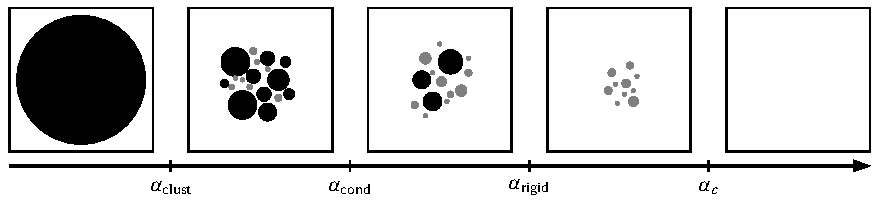
\includegraphics[width=1\textwidth]{figures/phase-transitions.pdf}
    \caption[Transitions de phase du problème SAT]{Schéma des transitions de phase du problème SAT selon le rapport du nombre de clauses au nombre de variables $\alpha$. Les transitions de phases illustrées sont la transition de regroupement $\alpha_{\text{clust}}$, la transition de condensation $\alpha_{\text{cond}}$, la transition de congélation $\alpha_{\text{rigid}}$ et la transition de satisfaisabilité $\alpha_{c}$. Figure tirée de~\cite{mooreNatureComputation2011}.}
    \label{fig:transitions-de-phase}
\end{figure}

Avant la première transition de phase située à $\alpha_{\text{clust}}$, la \textit{transition de phase de regroupement}, toutes les solutions d'une instance du problème SAT sont situées au sein du même amas. Après cette transition, un nombre exponentiel d'amas font leur apparition, séparés par une grande distance d'Hamming. Deux autres transitions apparaissent aussi en augmentant la densité des clauses sur les variables. Après la \textit{transition de phase de condensation} à $\alpha_{\text{cond}}$, un nombre sous-exponentiel d'amas domine l'ensemble de solutions. Finalement, les variables de chaque amas sont forcées de prendre des valeurs particulières après la \textit{transition de phase de congélation} à $\alpha_{\text{rigid}}$.

Les approches locales échouent à la transition de condensation en raison de la présence de corrélations à longues distances, comme mis en évidence par la méthode de propagation des convictions~\cite{mezardInformationPhysicsComputation2009}. La propagation par sondage corrige la propagation des convictions en adressant les corrélations à longues distances et permet de localiser la transition de congélation suivant la transition de condensation~\cite{mezardInformationPhysicsComputation2009}. Ces méthodes suggèrent que la difficulté du problème SAT provient de la transition de congélation. 

La transition de phase critique pour NAE3SAT est située à $\alpha_{c} \approx 2.1$~\cite{achlioptasPhaseTransition1ink2001} et à $\alpha_{c} \approx 2/3$~\cite{raymondPhaseDiagram1in32007} pour 1-in-3SAT. Les problèmes \#SAT semblent quant à eux être aussi maximalement complexes près de la phase de satisfaisabilité~\cite{dyerMarkovChainsIndependent2000, barthelClusteringAnalysisGroundstate2004}. Les instances du problème \#1-in-3SAT près du seuil critique appartiennent à la catégorie des problèmes bloqués, où la distance de Hamming entre n'importe quelles solutions est de $O(n)$. Ceux-ci font partis des problèmes les plus difficiles de la classe \textsf{\#P}~\cite{zdeborovaStatisticalPhysicsHard2008}.

L'approche utilisée dans le travail de ce mémoire se base sur l'optimisation des paramètres de circuits quantiques. Cette approche n'est pas locale comme avec les algorithmes classiques typiquement utilisés, ce qui laisse ainsi espérer un possible avantage. Par exemple, le problème \#XORSAT est résoluble avec une méthode globale, l'élimination gaussienne, en temps polynomial~\cite{mooreNatureComputation2011}.
